%Chapter 03
%************************************************
\chapter{Planning Algorithms}\label{ch:planningalgorithms}
%************************************************
Overview and classification of path planning algorithms
\section{Global Planning}\label{sec:global}
\subsection{Graph Search}
\subsubsection{Breadth-First Search (BFS)}
\subsubsection{Depth-First Search (DFS)}
\subsubsection{Dijkstra's and A* algorithm}
An illustration is given in Figure~\ref{fig:fig_overview}
\begin{figure}[thpb]
	  \myfloatalign
      \footnotesize
      \centering
    \subfloat[Dijkstra algorithm]
    {  \label{fig:fig_djikstra}
        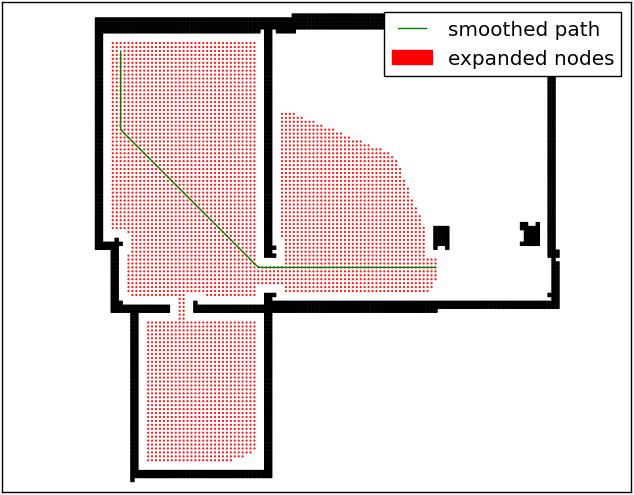
\includegraphics[width=0.75\textwidth]{figures/fig_djikstra.png}
        %\caption{Dijkstra}
    }
    
    \subfloat[A* algorithm]
    {  \label{fig:fig_astar}
       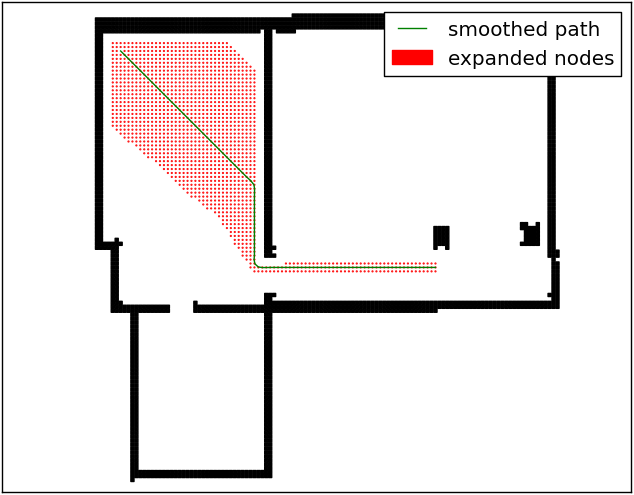
\includegraphics[width=0.75\textwidth]{figures/fig_astar.png}
       %\caption{A*}
    }
   \caption[Djikstra's and A* algorithm.]{The difference between Djikstra's and A* algorithm searching for a shortest path in a grid representation of a building. A* is more effective, as it visits by far less nodes in the search graph. }
   \label{fig:fig_overview}
\end{figure}
\subsection{Roadmap Based Navigation}
\subsubsection{Rapidly Exploring Randomized Trees (RRT)}
\subsubsection{Probabilistic Road Maps (PRM)}
\subsection{Potential Field}

\section{Local Planning and Obstacle Avoidance}\label{sec:local}
\subsection{Bug Algorithms}

M. I. Ribeiro. Obstacle avoidance. Institute for Systems and Robotics, [Online], Available:  \url{http://users.isr.ist.utl.pt/~mir/}, March 5, 2011.

\subsection{Vector Field Histogram(VFH)}

\subsection{Nearness Diagrams (ND)}
original Nearness Diagram \cite{minguez2004nearness}, and improved versions ND+ \cite{minguez2004divide} and Smooth Nearness Diagram (SND) \cite{durham2008smooth}.

\subsection{Curvature Velocity Method (CVM)}
The Curvature Velocity Method in \cite{simmons1996curvature} describes an obstacle avoidance method which considers kinematic and dynamic constraints of the robot and the environment.
These constraints are added to a \emph{velocity space} which consists of \emph{translational velocity} $v$ and \emph{rotational velocity} $w$.
One basic assumption of this approach is that the robot can only travel along circles with curvature $c=w/v$. 
This approximation neglects acceleration issues and restricts the robot motions to constant velocities over a given time horizon. 
  
Another simplification is the representation of obstacles as circles, which is used for fast transformation of the obstacles into the velocity space.
All curvatures which do not hit obstacles and adhere to the kinematic constraints of the robot are then evaluated using a cost function.
Since approximation techniques like simulated annealing to maximize the cost function using the whole velocity space did not succeed, the velocity space is divided into finite sets of curvature intervals.
The objective function is then evaluated over all curvature intervals.

A problem of this method arises when confronted with narrow passages which are perpendicular to the robots heading, which might lead to missing shorter paths. 
This problem is solved by the Lane Curvature Method \cite{ko1998lane}, by
dividing the workspace into finite number of lanes. 
The best angular velocity for changing lanes is evaluated using the CVM method. 

\subsection{Dynamic Window Approach (DWA)}\label{sec:dwa}
A well known method for local planning is the Dynamic Window Approach proposed in \cite{DWA1997}. 
The method samples the \emph{velocity space} $(v,w)$ of the robot, where again $v$ is the \emph{linear velocity} and $w$ the \emph{angular velocity} of the robot, to create a set of feasible trajectories.
The space is reduced to a \emph{dynamic window} which contains the reachable minimal and maximal velocity in one control cycle, taken the acceleration limits of the robot into account.

Obstacles are transformed into the velocity space using a distance function.
Figure \ref{fig:fig_dynamic} shows the obstacles in velocity space and the corresponding dynamic window. 
\begin{figure}[thpb]
	  \myfloatalign
      \scriptsize
      \centering
    \subfloat
    {  
       \def\svgwidth{0.75\textwidth}
       \includesvg{figures/fig_dynamic}
    } 
   \caption[Dynamic Window]{This Figure shows a dynamic window $V_d$ of a robot together with obstacles transformed in to a velocity space $V_s$. Only the velocities within the small area around the current robots speed $V_r$ are used for evaluating trajectories by a cost function. The best velocities are forwareded to the robots motor controller. (reproduced from \cite{DWA1997})}
   \label{fig:fig_dynamic}
\end{figure}


For a fixed amount of velocity samples the corresponding trajectories are created using a predefined granularity by performing forward simulation for a short period of time, starting at the current position and speed of the robot. 
The trajectories which stop safely before an obstacles are called \emph{feasible}.
Evaluating all \emph{feasible} trajectories with respect to a weighted cost function (cf. Equation~\ref{eq:costfunction}) identifies the best velocity tuple, which is then forwarded to the motor controller.

\begin{equation}
   f_c(v,w)=\alpha f_a(v,w)+\beta f_d(v,w)+\gamma f_v(v,w)
   \label{eq:costfunction}
\end{equation}

The function $f_a(v,w)$ judges the angle between the robots heading and a given goal position.
It is maximal if the heading is a straight line to the goal.
The distance to the closest obstacle is calculated in the function $f_d(v,w)$.
The function $f_v(v,w)$ takes the forward velocity into account and rewards faster movements of the robot.

In this method the obstacles are not approximated by circles, instead small lines are used to account for a more accurate representation of obstacles.
The robot is still approximated as a circle.
The original method does not use a global plan to guide the robot, so without further changes it is subject to get captured in local minima.

Other applications of this approach in recent planning systems adapt the corresponding cost function. 
%give some recent papers about dwa in developments%
The excellent \texttt{move\_base}\footnote{move\_base planning framework: \url{http://wiki.ros.org/move_base}} motion planning framework introduced in \cite{DBLP:conf/icra/Marder-EppsteinBFGK10} implements within the navigation stack of Robot Operating System (ROS) a local planner which uses a global plan as a guide, and uses a polygon to model the robot outline.

One implementation is based on DWA.
There is also the option to use Trajectory rollout \cite{gerkey08planning} as a local planner which is very related to the DWA, but in contrast improves in simulating the robots trajectory by accurately applying acceleration limits over the whole simulation time.
The cost function maximizes characteristics like proximity to obstacles, proximity to the goal, proximity to the global path, and speed.
Furthermore a number of escaping strategies try to avoid the vulnerability to local minima. 

Collision detection and cost calculation is performed by using the footprint of the robot following the calculated trajectory.
Hence the discretized footprint, which is usually given as a simple polygon, is projected on the costmap. 
Bresenham's Line algorithm \cite{bresenham1965algorithm} is used for ray-tracing the contour of a robot in the discrete workspace. 
Figure~\ref{fig:fig_global} shows the global view of the planning task. 
In Figure~\ref{fig:fig_local} the corresponding local view is depicted, including all sampled trajectories which are evaluated using a local costmap.

\begin{figure}[thpb]
	  \myfloatalign
      \footnotesize
      \centering
    \subfloat[Path planning in global costmap.]
    {  \label{fig:fig_global}
       \def\svgwidth{0.75\textwidth}
       \includesvg{figures/fig_global}

    } \\    
    \subfloat[Trajectory generation for linear, and angular velocities $(v,w)$ in local costmap guided by global path.]
    {  \label{fig:fig_local}
       \def\svgwidth{0.75\textwidth}
       \includesvg{figures/fig_local}
    }
   \caption[]{}
   \label{fig:fig_dwa}
\end{figure}

Concerning the optimization of the used cost functions the most common approach for DWA and related local planner is to evaluate all possible trajectories in a reduced discrete velocity space. 
Examples of this approach can be found in \cite{kiss2012advanced}\cite{DBLP:conf/icra/Marder-EppsteinBFGK10}\cite{conf/icra/SederP07}. 

The proposed method extends the DWA approach, by using approximation algorithm to maximize the cost function in a discrete representation of the velocity space.

%*****************************************
%*****************************************
%*****************************************
%*****************************************
%*****************************************




